% !TEX root = main.tex
\documentclass[12pt,a4paper]{ltjsarticle}

%% Fonts
\usepackage{lmodern}
\usepackage{luatexja-preset}

%% Layout
\usepackage[top=30mm, bottom=25mm, left=25mm, right=25mm]{geometry}
%% Section heading spacing — reduce vertical space before/after \section and \subsection.
%% Use the starred (*) versions to suppress paragraph indentation after the heading.
\usepackage{titlesec}
\titlespacing{\section}{0pt}{3.5ex plus 1ex minus 0.5ex}{2.3ex plus 0.5ex}
\titlespacing{\subsection}{0pt}{3.25ex plus 1ex minus 0.5ex}{1.5ex plus 0.5ex}

%% Color / graphics
\usepackage[svgnames,table]{xcolor}
\usepackage{graphicx}
\usepackage{float}

%% Diagrams / charts
\usepackage{tikz}
\usetikzlibrary{calc}
\usepackage{pgfplots}
\pgfplotsset{compat=1.18}

%% Source code listings
\usepackage{listings}
\renewcommand{\lstlistingname}{ソースコード}

%% Hyperlinks (load near last)
\usepackage{hyperref}

%% Header / footer
\usepackage{fancyhdr}

%% Captions
\usepackage[format=hang, font=small, labelfont=bf]{caption}
\usepackage{subcaption}

%% Mathematics
\usepackage{amsmath}
\usepackage{amssymb}

%% Professional table rules
\usepackage{booktabs}

%% URL
\usepackage{url}

%% List customization
\usepackage{enumitem}

%% Wide tables
\usepackage{tabularx}
\usepackage{multirow}

%% ── Source Code Appearance ───────────────────────────────────
\definecolor{codebg}{RGB}{248,248,248}
\definecolor{codeframe}{RGB}{180,180,180}
\definecolor{kwcolor}{RGB}{0,0,180}
\definecolor{cmcolor}{RGB}{100,100,100}
\definecolor{stcolor}{RGB}{160,0,0}

\lstset{
  backgroundcolor  = \color{codebg},
  basicstyle       = \ttfamily\small,
  keywordstyle     = \color{kwcolor}\bfseries,
  commentstyle     = \color{cmcolor}\itshape,
  stringstyle      = \color{stcolor},
  numbers          = left,
  numberstyle      = \tiny\color{gray},
  numbersep        = 8pt,
  frame            = single,
  rulecolor        = \color{codeframe},
  breaklines       = true,
  breakatwhitespace= false,
  showstringspaces = false,
  tabsize          = 4,
  captionpos       = b,
  xleftmargin      = 2em,
  framexleftmargin = 1.5em,
}

%% ── Page Style ───────────────────────────────────────────────
\pagestyle{fancy}
\fancyhf{}
\rhead{\small プログラミング実験}
\lhead{\small \nouppercase{\leftmark}}
\cfoot{\thepage}
\renewcommand{\headrulewidth}{0.4pt}

\fancypagestyle{titlepage}{
  \fancyhf{}
  \renewcommand{\headrulewidth}{0pt}
}
\fancypagestyle{frontmatter}{
  \fancyhf{}
  \cfoot{\thepage}
  \renewcommand{\headrulewidth}{0pt}
}

%% ── Hyperlink / PDF metadata ─────────────────────────────────
\hypersetup{
  colorlinks = true,
  linkcolor  = NavyBlue,
  citecolor  = NavyBlue,
  urlcolor   = NavyBlue,
  pdftitle   = {統計データ処理レポート},
  pdfauthor  = {Deka Risman Permana},
  pdfsubject = {プログラミング実験},
  pdfkeywords= {人間情報システム工学科 4年},
}

\newcommand{\HRule}{\rule{\linewidth}{0.5mm}}

\title{}
\date{}
\author{}

%% ============================================================
\begin{document}
%% ============================================================

%% ── Title Page ───────────────────────────────────────────────
\begin{titlepage}
\setlength{\parindent}{0pt}
  
\begin{center}
{\huge \textbf{情報工学実験Ⅱレポート（山本担当分）表紙}}\\[0.8cm]
\end{center}

\begin{large}
番号： 4347 名前： Deka Risman Permana\vspace{0.3cm}

実施日時： 令和8年4月29日、5月13日 場所： HIパソコン室\vspace{0.3cm}

提出〆切： 令和8年5月20日（水）8:50 WebClass\vspace{0.3cm}

実験テーマ名：（第3、4回）統計データ処理\vspace{0.3cm}

チェック欄： 次表の項目について自己チェックしてください
\end{large}

\begin{center}
\begin{tabularx}{\textwidth}{|X|>{\centering\arraybackslash}m{5cm}|}
  \hline
  \multicolumn{1}{|c|}{\multirow{2}{*}{\textbf{項目}}} & \textbf{自己チェック} \\
  & \textbf{（出来たものに◯をつける）} \\
  \hline
  実験目的がある & ◯\\
  \hline
  （問題1）「1変量データの要約」の課題1について、スクリプト、実行結果、説明がついている & ◯\\
  \hline
  （問題1）「1変量データの要約」の課題2について、スクリプト、実行結果、説明がついている & ◯\\
  \hline
  （問題1）「ベクトルデータの操作」の課題1について、スクリプト、実行結果、説明がついている & ◯\\
  \hline
  （問題1）「表データの操作」の課題1について、スクリプト、実行結果、説明がついている & ◯\\
  \hline
  （問題1）「表データの操作」の課題2について、スクリプト、実行結果、説明がついている & ◯\\
  \hline
  （問題2(a)）この課題について、ER図をつけ、その説明もついている & ◯\\
  \hline
  （問題2(b)）この課題について、スクリプト、実行結果、説明がついている & ◯\\
  \hline
  （問題2(c)）追加した機能のテーブル例と追加分を含む全体のER図をつけ、それらの説明もついている & ◯\\
  \hline
  感想がある & ◯\\
  \hline
  参考文献がある & ◯\\
  \hline
  レポートの1枚目にこの表紙をつけている & ◯\\
  \hline
\end{tabularx}
\end{center}
  
\end{titlepage}

%% ── Table of Contents ────────────────────────────────────────
\newpage
\thispagestyle{frontmatter}
\pagenumbering{roman}
\tableofcontents

\newpage
\pagenumbering{arabic}
\setcounter{page}{1}

%% ── Sections ─────────────────────────────────────────────────

\section{実験目的}\label{sec:objective}
R の統計処理に関するプログラミングを理解し、統計データの処理ができる。また、データモデルに関
する基本的な概念を説明できる。

\section{問題1：統計データ処理}\label{sec:problem1}

%% ============================================================
\subsection{1変量データの要約}\label{sec:univariate}

データを入手したらまず最初にデータ全体を見渡す「データレビュー」が必要である。本節では
\texttt{demodata.csv}の各変数に対して、ヒストグラムとボックスプロットを用いてデータの
分布を可視化し、要約統計量を計算する。

量的変数の要約には「平均と標準偏差」または「中央値と四分位範囲」を用いる。ヒストグラムは
区切り方によって見え方が変わるため、外れ値に強いボックスプロットも併用することが重要で
ある。

%% ------------------------------------------------------------
\subsubsection{課題1：各変数のヒストグラムとボックスプロット}\label{sec:univariate-task1}

\texttt{demodata.csv}に含まれる以下の8変数について、ヒストグラムとボックスプロットを
描画した。

%% R スクリプト -------------------------------------------------
\lstinputlisting[
    language=R,
    caption={課題1のRスクリプト：ヒストグラムとボックスプロット},
    label={lst:univariate-task1}
]{code/task1-1.R}

%% 図 ------------------------------------------------------------
\begin{figure}[H]
    \centering
    \begin{subfigure}[b]{0.48\textwidth}
        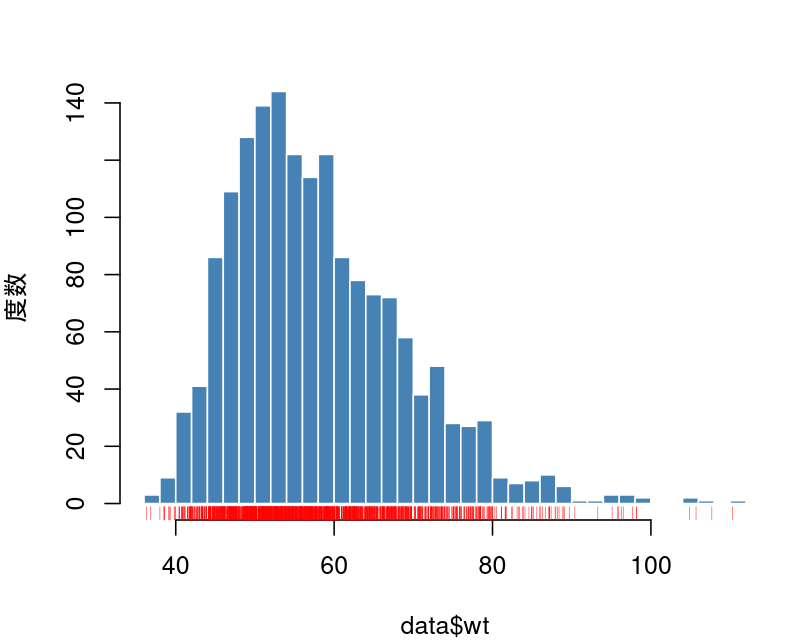
\includegraphics[width=\textwidth]{images/hist_wt.png}
        \caption{体重のヒストグラム}
        \label{fig:hist-wt}
    \end{subfigure}
    \hfill
    \begin{subfigure}[b]{0.48\textwidth}
        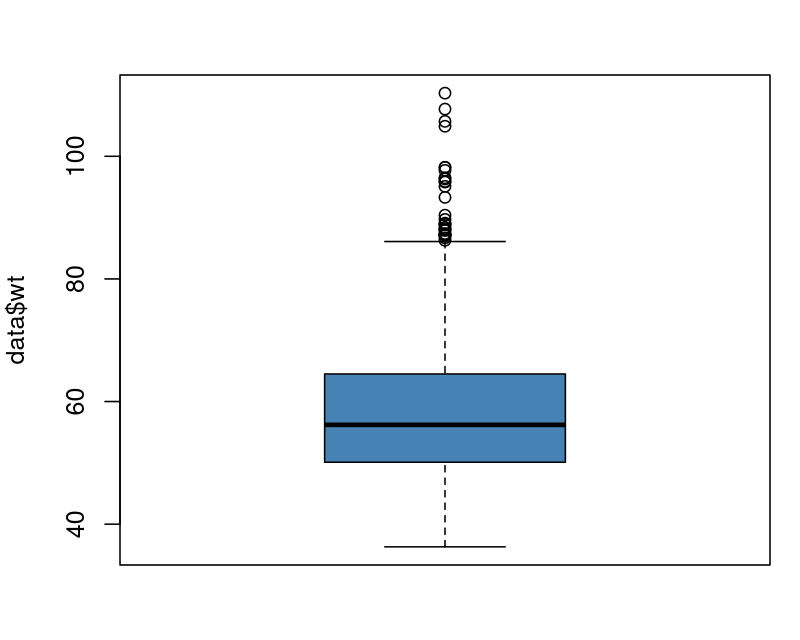
\includegraphics[width=\textwidth]{images/boxplot_wt.png}
        \caption{体重のボックスプロット}
        \label{fig:boxplot-wt}
    \end{subfigure}
    \caption{体重（wt）の分布}
    \label{fig:univariate-wt}
\end{figure}
\vspace{-3.2em}

\begin{figure}[H]
    \centering
    \begin{subfigure}[b]{0.48\textwidth}
        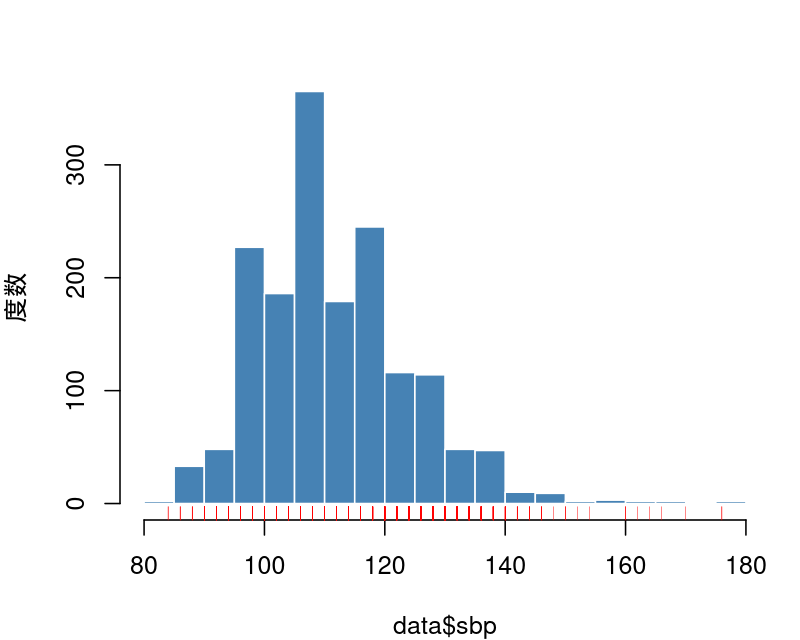
\includegraphics[width=\textwidth]{images/hist_sbp.png}
        \caption{収縮期血圧のヒストグラム}
        \label{fig:hist-sbp}
    \end{subfigure}
    \hfill
    \begin{subfigure}[b]{0.48\textwidth}
        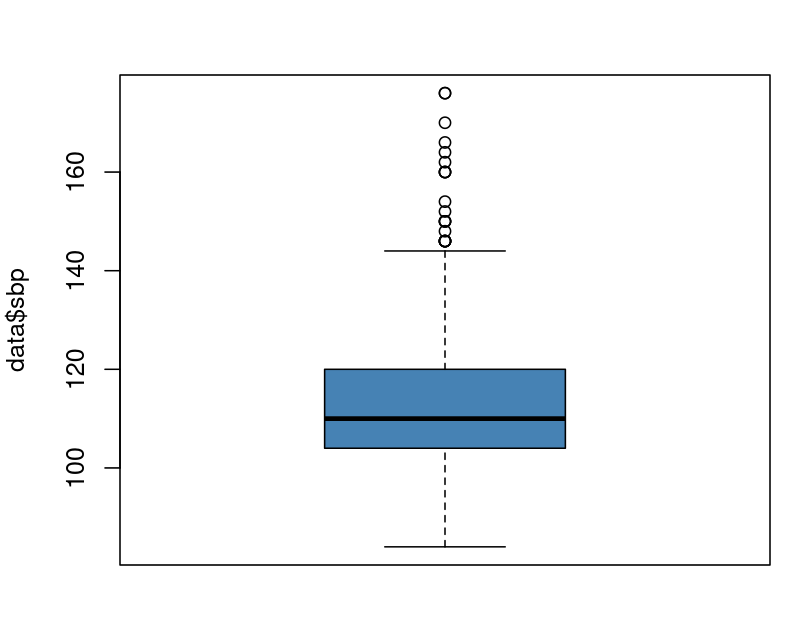
\includegraphics[width=\textwidth]{images/boxplot_sbp.png}
        \caption{収縮期血圧のボックスプロット}
        \label{fig:boxplot-sbp}
    \end{subfigure}
    \caption{収縮期血圧（sbp）の分布}
    \label{fig:univariate-sbp}
\end{figure}
\vspace{-3.2em}

\begin{figure}[H]
    \centering
    \begin{subfigure}[b]{0.48\textwidth}
        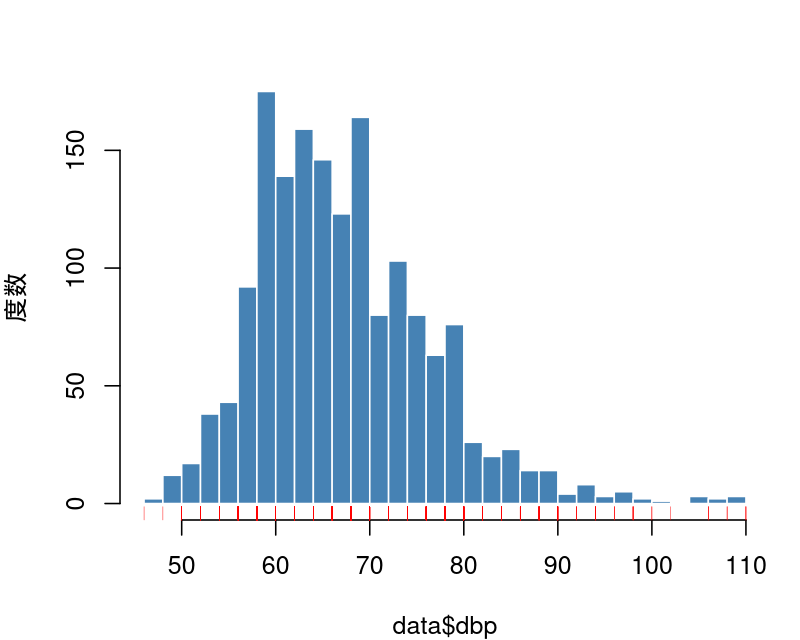
\includegraphics[width=\textwidth]{images/hist_dbp.png}
        \caption{拡張期血圧のヒストグラム}
        \label{fig:hist-dbp}
    \end{subfigure}
    \hfill
    \begin{subfigure}[b]{0.48\textwidth}
        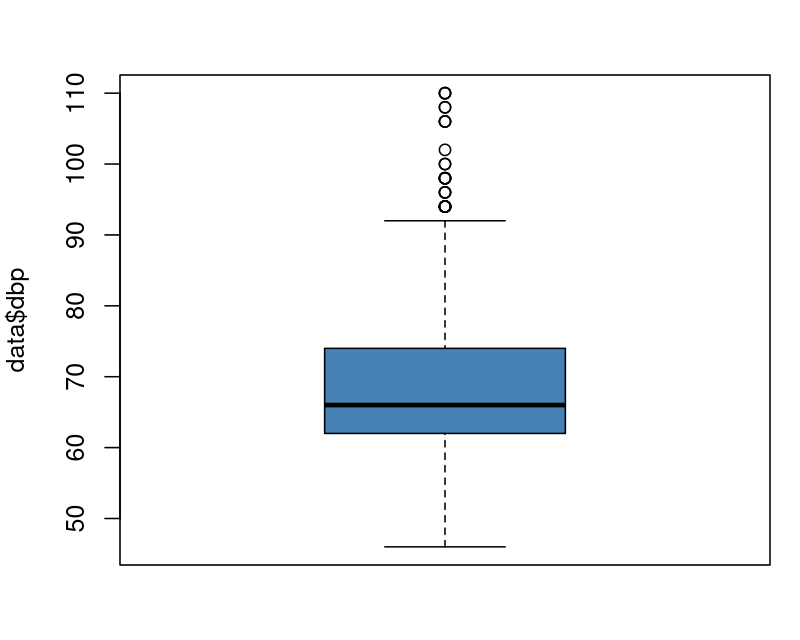
\includegraphics[width=\textwidth]{images/boxplot_dbp.png}
        \caption{拡張期血圧のボックスプロット}
        \label{fig:boxplot-dbp}
    \end{subfigure}
    \caption{拡張期血圧（dbp）の分布}
    \label{fig:univariate-dbp}
\end{figure}
\vspace{-3.2em}

\begin{figure}[H]
    \centering
    \begin{subfigure}[b]{0.48\textwidth}
        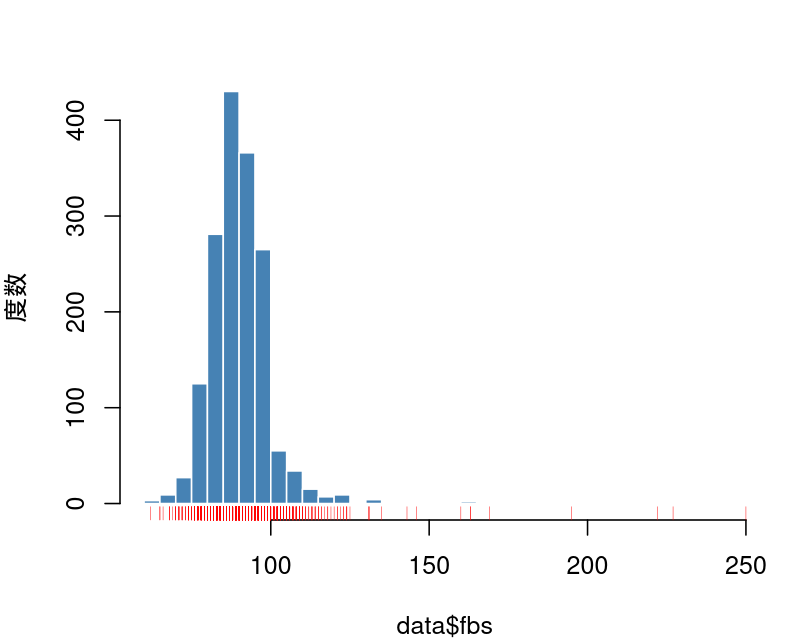
\includegraphics[width=\textwidth]{images/hist_fbs.png}
        \caption{空腹時血糖のヒストグラム}
        \label{fig:hist-fbs}
    \end{subfigure}
    \hfill
    \begin{subfigure}[b]{0.48\textwidth}
        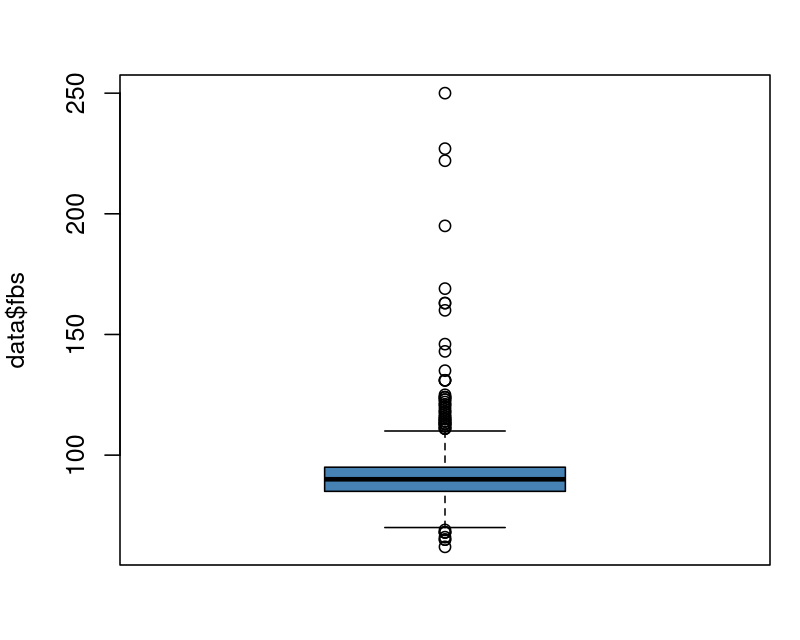
\includegraphics[width=\textwidth]{images/boxplot_fbs.png}
        \caption{空腹時血糖のボックスプロット}
        \label{fig:boxplot-fbs}
    \end{subfigure}
    \caption{空腹時血糖（fbs）の分布}
    \label{fig:univariate-fbs}
\end{figure}
\vspace{-3.2em}

\begin{figure}[H]
    \centering
    \begin{subfigure}[b]{0.48\textwidth}
        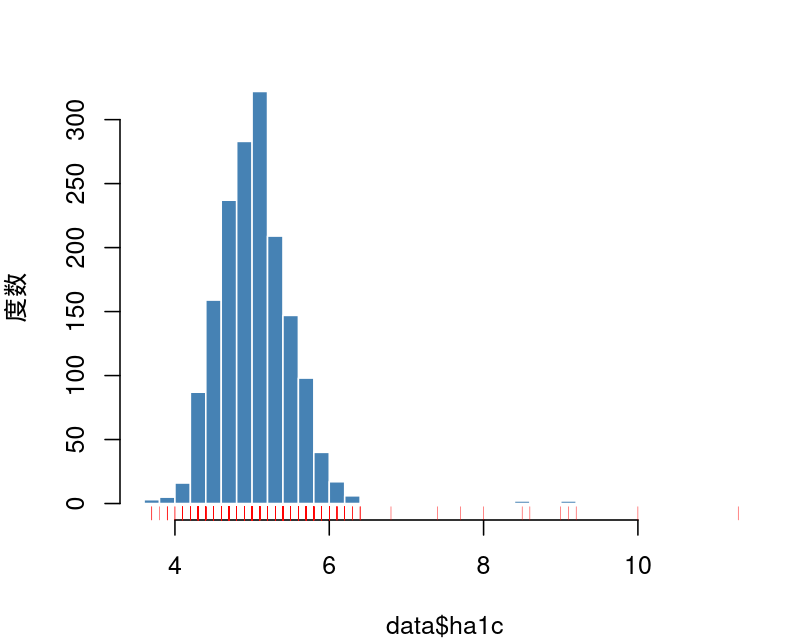
\includegraphics[width=\textwidth]{images/hist_ha1c.png}
        \caption{ヘモグロビンA1cのヒストグラム}
        \label{fig:hist-ha1c}
    \end{subfigure}
    \hfill
    \begin{subfigure}[b]{0.48\textwidth}
        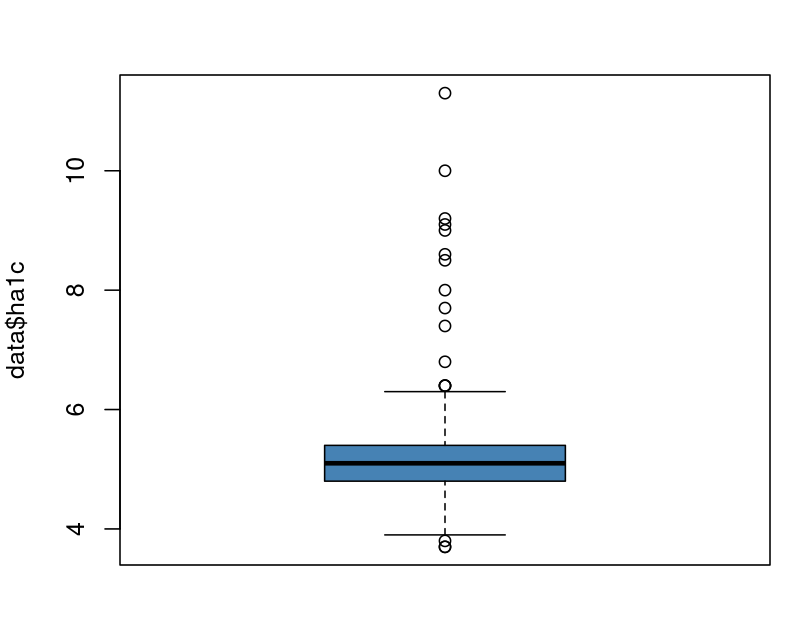
\includegraphics[width=\textwidth]{images/boxplot_ha1c.png}
        \caption{ヘモグロビンA1cのボックスプロット}
        \label{fig:boxplot-ha1c}
    \end{subfigure}
    \caption{ヘモグロビンA1c（ha1c）の分布}
    \label{fig:univariate-ha1c}
\end{figure}
\vspace{-3.2em}

\begin{figure}[H]
    \centering
    \begin{subfigure}[b]{0.48\textwidth}
        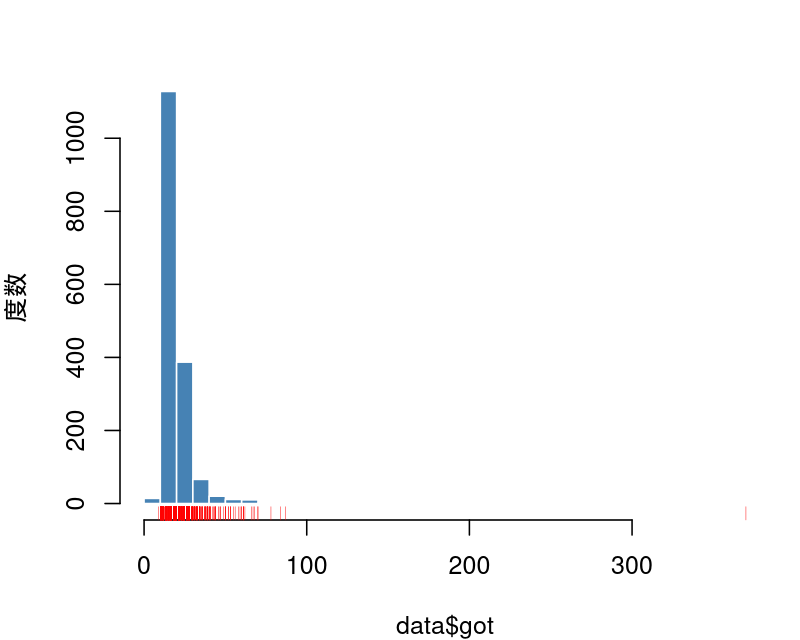
\includegraphics[width=\textwidth]{images/hist_got.png}
        \caption{GOTのヒストグラム}
        \label{fig:hist-got}
    \end{subfigure}
    \hfill
    \begin{subfigure}[b]{0.48\textwidth}
        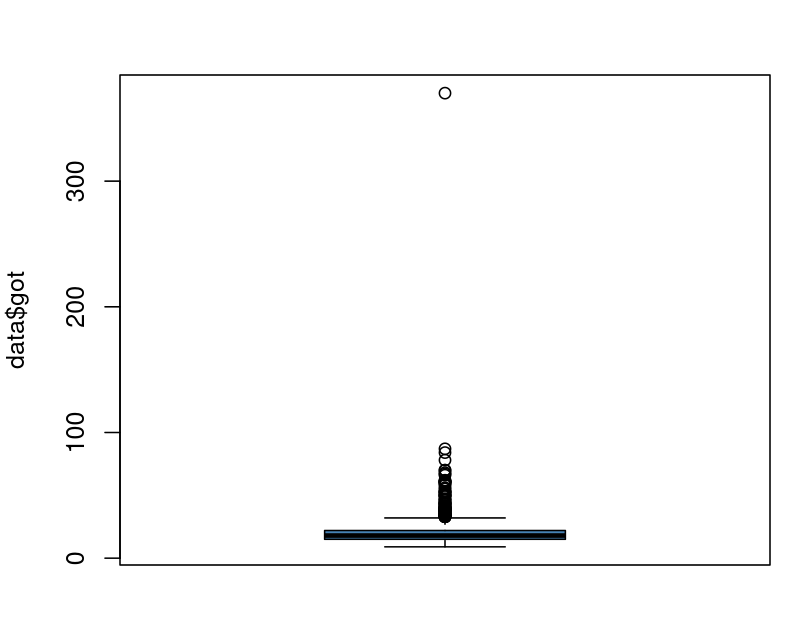
\includegraphics[width=\textwidth]{images/boxplot_got.png}
        \caption{GOTのボックスプロット}
        \label{fig:boxplot-got}
    \end{subfigure}
    \caption{GOT（got）の分布}
    \label{fig:univariate-got}
\end{figure}
\vspace{-3.2em}

\begin{figure}[H]
    \centering
    \begin{subfigure}[b]{0.48\textwidth}
        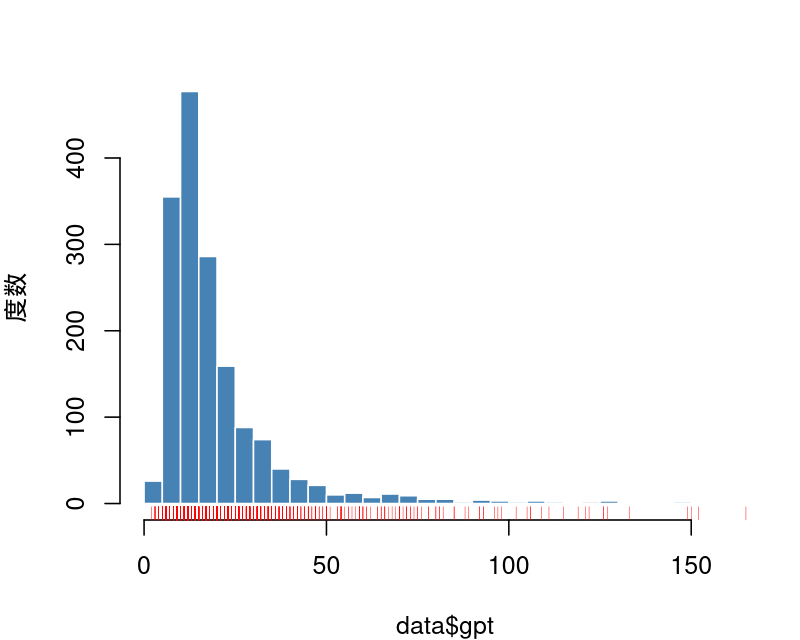
\includegraphics[width=\textwidth]{images/hist_gpt.png}
        \caption{GPTのヒストグラム}
        \label{fig:hist-gpt}
    \end{subfigure}
    \hfill
    \begin{subfigure}[b]{0.48\textwidth}
        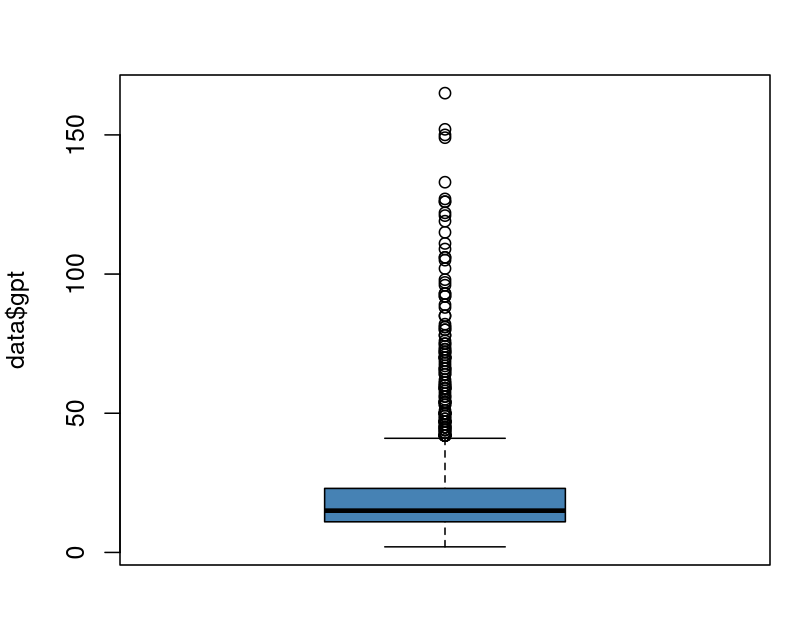
\includegraphics[width=\textwidth]{images/boxplot_gpt.png}
        \caption{GPTのボックスプロット}
        \label{fig:boxplot-gpt}
    \end{subfigure}
    \caption{GPT（gpt）の分布}
    \label{fig:univariate-gpt}
\end{figure}
\vspace{-3.2em}

\begin{figure}[H]
    \centering
    \begin{subfigure}[b]{0.48\textwidth}
        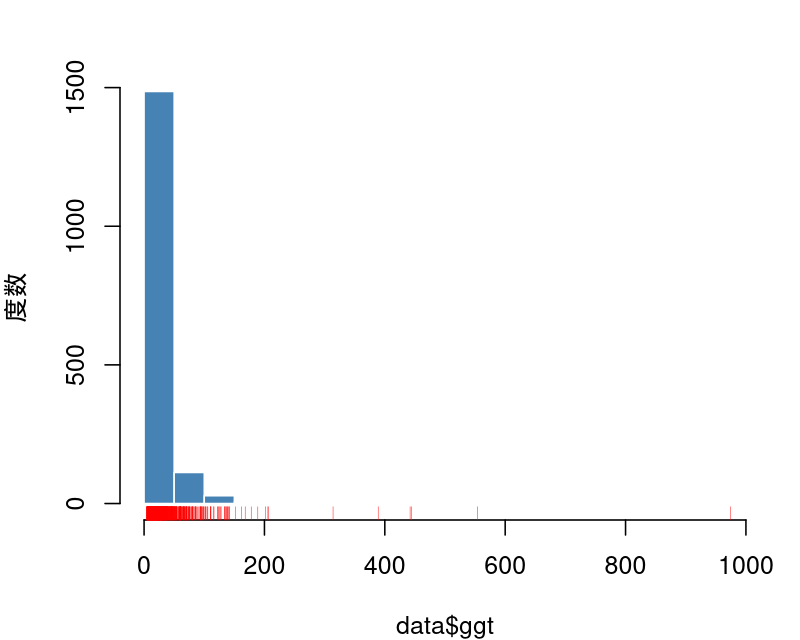
\includegraphics[width=\textwidth]{images/hist_ggt.png}
        \caption{$\gamma$-GTPのヒストグラム}
        \label{fig:hist-ggt}
    \end{subfigure}
    \hfill
    \begin{subfigure}[b]{0.48\textwidth}
        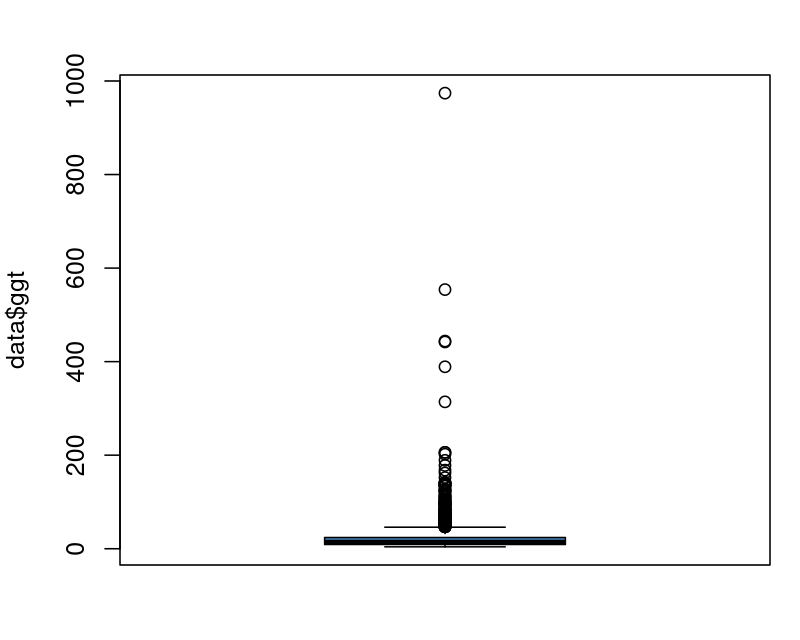
\includegraphics[width=\textwidth]{images/boxplot_ggt.png}
        \caption{$\gamma$-GTPのボックスプロット}
        \label{fig:boxplot-ggt}
    \end{subfigure}
    \caption{$\gamma$-GTP（ggt）の分布}
    \label{fig:univariate-ggt}
\end{figure}

%% ------------------------------------------------------------
\subsubsection{課題2：動脈硬化指数（AI）}\label{sec:univariate-task2}

動脈硬化指数（Atherogenic Index: AI）は以下の式で定義される。

\begin{equation}
    \text{AI} = \frac{\text{TC} - \text{HDLc}}{\text{HDLc}}
    \label{eq:ai}
\end{equation}

ここで、TCは総コレステロール（\texttt{tc}）、HDLcはHDLコレステロール（\texttt{hdlc}）
である。この指数の要約統計量（平均、標準偏差、中央値、四分位範囲、最小値、最大値）を求め、
ヒストグラムとボックスプロットを描画した。

\lstinputlisting[
    language=R,
    caption={課題2のRスクリプト：AI指数の計算と可視化},
    label={lst:univariate-task2}
]{code/task1-2.R}

\begin{table}[htbp]
    \centering
    \caption{動脈硬化指数（AI）の要約統計量}
    \label{tab:ai-summary}
    \begin{tabular}{lr}
        \toprule
        要約統計量 & 値 \\
        \midrule
        標本数 (n)          & 1,640 \\
        平均                & 4.103 \\
        標準偏差            & 7.079 \\
        中央値              & 4.048 \\
        第1四分位数 (Q1)    & 3.039 \\
        第3四分位数 (Q3)    & 5.194 \\
        四分位範囲 (IQR)     & 2.155 \\
        最小値              & 1.875 \\
        最大値              & 13.556 \\
        \bottomrule
    \end{tabular}
\end{table}

\begin{figure}[H]
    \centering
    \begin{subfigure}[b]{0.48\textwidth}
        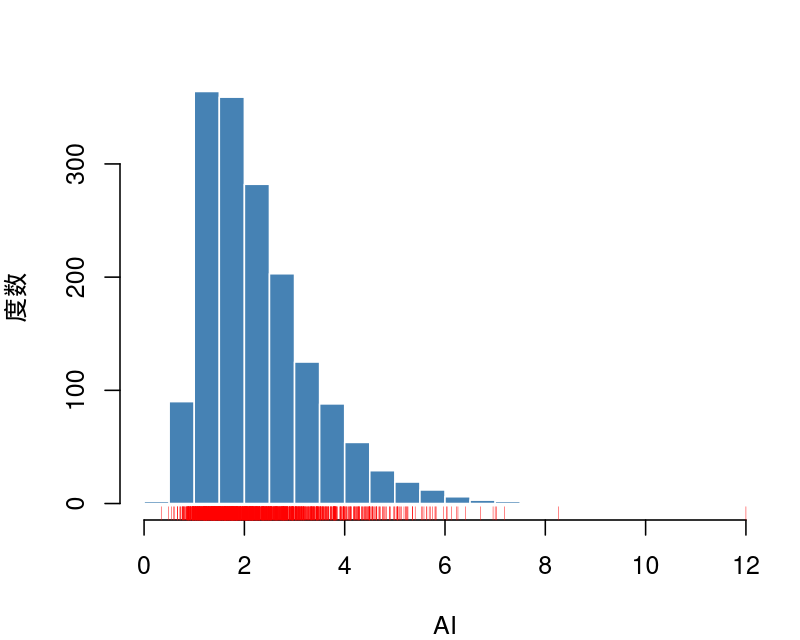
\includegraphics[width=\textwidth]{images/hist_ai.png}
        \caption{AIのヒストグラム}
        \label{fig:hist-ai}
    \end{subfigure}
    \hfill
    \begin{subfigure}[b]{0.48\textwidth}
        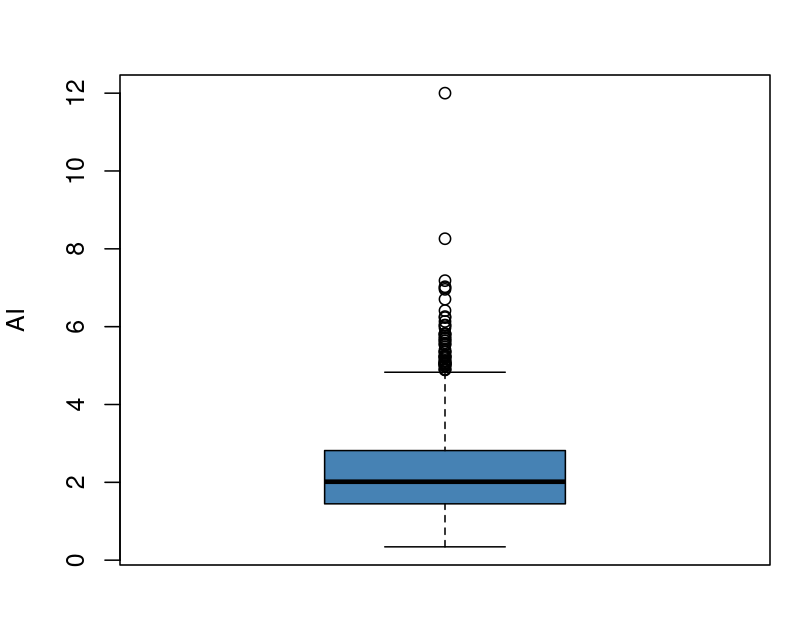
\includegraphics[width=\textwidth]{images/boxplot_ai.png}
        \caption{AIのボックスプロット}
        \label{fig:boxplot-ai}
    \end{subfigure}
    \caption{動脈硬化指数（AI）の分布}
    \label{fig:univariate-ai}
\end{figure}

\clearpage

%% ============================================================
\subsection{ベクトルデータの操作}\label{sec:vector}

Rにおけるベクトルデータの基本的な操作方法について理解する。ベクトルはRの最も基本的な
データ構造であり、同一型の要素を1次元に並べたものである。

%% ------------------------------------------------------------
\subsubsection{課題1：ベクトル操作}\label{sec:vector-task1}
\texttt{x <- c(1,2,3,4,5,6)}のなかで、以下の条件式を満たす成分を取り出す式と結果を記しなさい。
\begin{enumerate}[nosep, label=(\arabic*)]
    \item 3 より大きく，5 より小さい
\begin{lstlisting}
x[x > 3 & x < 5]
\end{lstlisting}
    
    \item 3 より小さいか，5 より大きい
\begin{lstlisting}
x[x < 3 | x > 5]
\end{lstlisting}

    \item 3 以下か，5 以上
\begin{lstlisting}
x[x <= 3 | x >= 5]
\end{lstlisting}

    \item 2 と 6 でない
\begin{lstlisting}
x[x != 2 & x != 6]
\end{lstlisting}

    \item 3 ではなく，かつ 1 以上 5 以下
\begin{lstlisting}
x[!(x == 3) & x >= 1 & x <= 5]
\end{lstlisting}
\end{enumerate}

\subsubsection*{説明}
Rでは、角括弧 \texttt{[]} の中に論理ベクトルを記述することで、\texttt{TRUE} に
対応する成分のみを取り出すことができる。論理演算子 \texttt{\&}（AND）、
\texttt{|}（OR）、\texttt{!}（NOT）を用いて複合条件を表現する。

\begin{itemize}[nosep]
    \item (1) \texttt{x > 3 \& x < 5} は「3より大きく、かつ5より小さい」成分を指定し、
          結果は \texttt{4} となる。
    \item (2) \texttt{x < 3 | x > 5} は「3より小さい、または5より大きい」成分を指定し、
          結果は \texttt{1, 2, 6} となる。
    \item (3) \texttt{x <= 3 | x >= 5} は「3以下、または5以上」の成分を指定し、
          結果は \texttt{1, 2, 3, 5, 6} となる。
    \item (4) \texttt{x != 2 \& x != 6} は「2でも6でもない」成分を指定し、
          結果は \texttt{1, 3, 4, 5} となる。
    \item (5) \texttt{!(x == 3) \& x >= 1 \& x <= 5} は「3ではなく、かつ1以上5以下」の
          成分を指定し、結果は \texttt{1, 2, 4, 5} となる。
\end{itemize}



\clearpage

%% ============================================================
\subsection{表データの操作}\label{sec:table}

RでCSVファイルを読み込むと表形式（データフレーム）として扱われる。列や行の取り出し、
条件による行の絞り込みなど、データフレーム操作の基本を習得する。

列の取り出しには\texttt{data\$変数名}、\texttt{data[ , 列番号]}、\texttt{data[ , "列名"]}
の3通りの方法がある。行の取り出しには\texttt{data[行番号, ]}または\texttt{data["行名", ]}
を用いる。条件に合う行のみを取り出すには\texttt{data[条件式, ]}と記述する。

%% ------------------------------------------------------------
\subsubsection{課題1：minidata.csvによるデータ抽出}\label{sec:table-task1}

\texttt{minidata.csv}（10人分の性別と身長のデータ）を用いて、以下の条件で行データを
抽出した。

\begin{enumerate}[nosep, label=(\arabic*)]
    \item 身長150cm未満の行データのみ抜き出す。
    \item 身長150cm以上、170cm未満の行データのみ抜き出す。
    \item 身長150cm以上、170cm未満で、女性のデータのみ抜き出す。
\end{enumerate}

%% R スクリプト -------------------------------------------------
\lstinputlisting[
    language=R,
    caption={課題1のRスクリプト：minidata.csvのデータ抽出},
    label={lst:table-task1}
]{code/task3-1.R}

%% 実行結果 ------------------------------------------------------
\lstinputlisting[
    language={},
    caption={minidata.csvからの条件抽出結果},
    label={lst:table-task1-result},
    numbers=none,
    basicstyle=\ttfamily\footnotesize
]{code/output_task3-1.txt}

\subsubsection*{説明}
\texttt{minidata.csv}には性別（\texttt{sex}）と身長（\texttt{ht}）の2変数が
10行格納されている。データフレームの行抽出には \texttt{data[条件式, ]} の
構文を用いる。

\begin{itemize}[nosep]
    \item (1) \texttt{data[data\$ht < 150, ]} により、身長150cm未満の2名
          （145.9cm, 147.2cm）が得られた。いずれも女性である。
    \item (2) \texttt{data[data\$ht >= 150 \& data\$ht < 170, ]} により、
          身長150cm以上170cm未満の5名が得られた。女性3名、男性2名が該当する。
    \item (3) (2)の条件に加えて \texttt{data\$sex == "f"} をAND条件で追加することで、
          身長150cm以上170cm未満の女性3名のみが抽出された。
\end{itemize}

%% ------------------------------------------------------------
\subsubsection{課題2：demodata.csvによる男女別分析}\label{sec:table-task2}

\texttt{demodata.csv}を用いて、男性と女性に分けた分析を行った。

\begin{enumerate}[nosep, label=(\arabic*)]
    \item 男性のデータを変数\texttt{mdata}、女性のデータを変数\texttt{fdata}に分割する。
    \item 男性の身長\texttt{ht}、体重\texttt{wt}、収縮期血圧\texttt{sbp}、拡張期血圧
          \texttt{dbp}のヒストグラムを描画する。
    \item 女性の身長\texttt{ht}、体重\texttt{wt}、収縮期血圧\texttt{sbp}、拡張期血圧
          \texttt{dbp}のヒストグラムを描画する。
    \item 男性の身長\texttt{ht}、体重\texttt{wt}、収縮期血圧\texttt{sbp}、拡張期血圧
          \texttt{dbp}の要約統計量（平均・標準偏差、中央値・四分位範囲）を求める。
    \item 女性の身長\texttt{ht}、体重\texttt{wt}、収縮期血圧\texttt{sbp}、拡張期血圧
          \texttt{dbp}の要約統計量（平均・標準偏差、中央値・四分位範囲）を求める。
\end{enumerate}

%% R スクリプト -------------------------------------------------
\lstinputlisting[
    language=R,
    caption={課題2のRスクリプト：demodata.csvの男女別分析},
    label={lst:table-task2}
]{code/task3-2.R}

%% データ分割 ----------------------------------------------------
\subsubsection*{データの分割結果}
\texttt{data[data\$sex == "m", ]} で男性行を抽出し \texttt{mdata}、
\texttt{data[data\$sex == "f", ]} で女性行を抽出し \texttt{fdata} とした。
\texttt{demodata.csv} の全1,640名のうち、男性は602名、女性は1,038名であった。

%% 図：男性のヒストグラム -----------------------------------------
\begin{figure}[H]
    \centering
    \begin{subfigure}[b]{0.48\textwidth}
        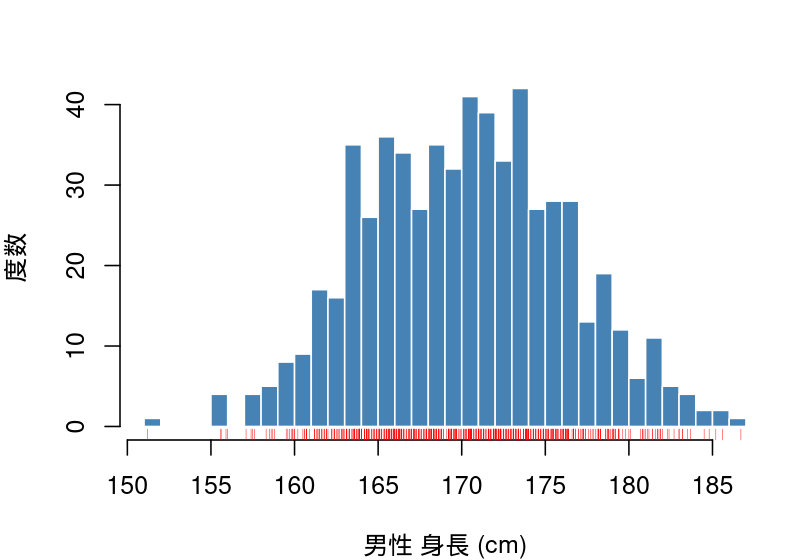
\includegraphics[width=\textwidth]{images/hist_m_ht.png}
        \caption{男性の身長}
        \label{fig:hist-m-ht}
    \end{subfigure}
    \hfill
    \begin{subfigure}[b]{0.48\textwidth}
        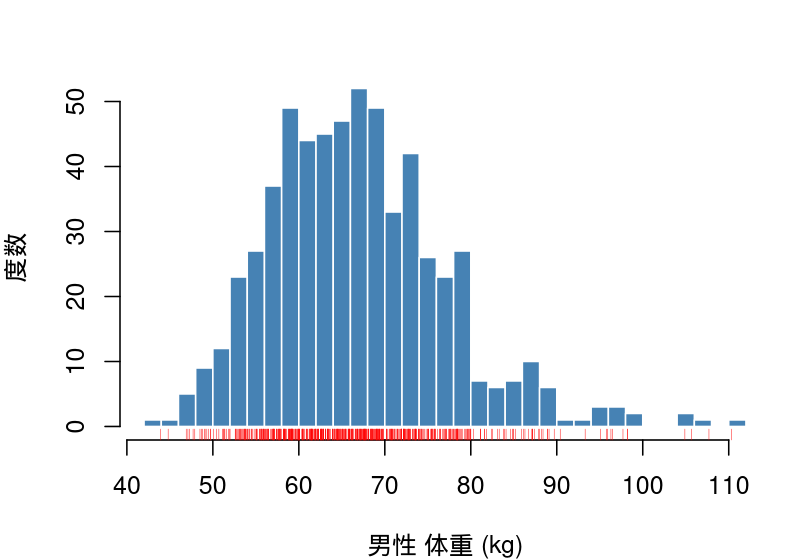
\includegraphics[width=\textwidth]{images/hist_m_wt.png}
        \caption{男性の体重}
        \label{fig:hist-m-wt}
    \end{subfigure}
    \caption{男性の身長・体重のヒストグラム}
    \label{fig:univariate-m-ht-wt}
\end{figure}
\vspace{-3.2em}

\begin{figure}[H]
    \centering
    \begin{subfigure}[b]{0.48\textwidth}
        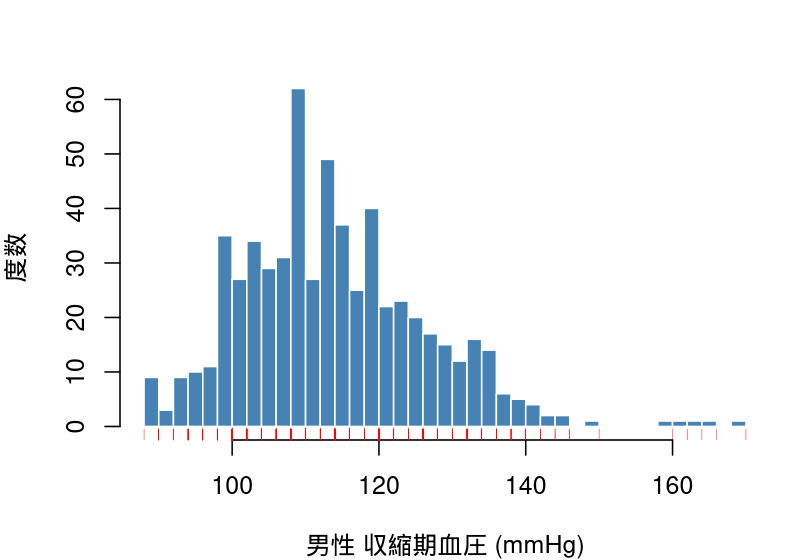
\includegraphics[width=\textwidth]{images/hist_m_sbp.png}
        \caption{男性の収縮期血圧}
        \label{fig:hist-m-sbp}
    \end{subfigure}
    \hfill
    \begin{subfigure}[b]{0.48\textwidth}
        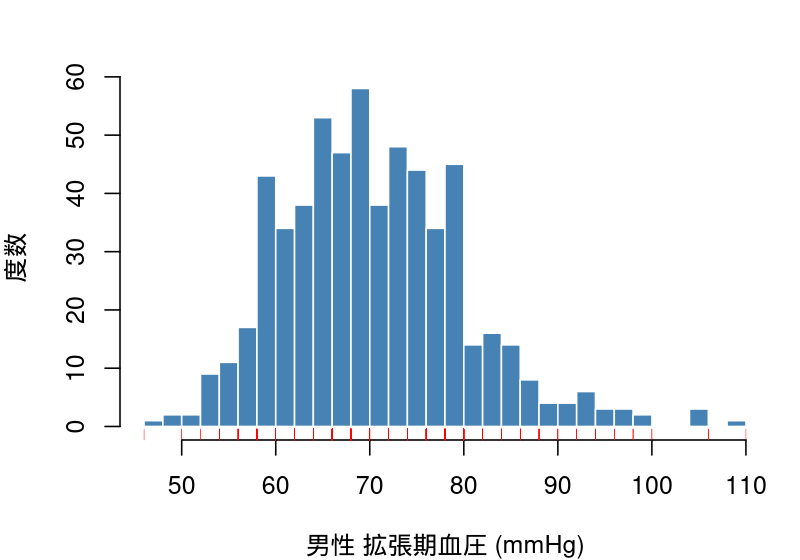
\includegraphics[width=\textwidth]{images/hist_m_dbp.png}
        \caption{男性の拡張期血圧}
        \label{fig:hist-m-dbp}
    \end{subfigure}
    \caption{男性の血圧のヒストグラム}
    \label{fig:univariate-m-bp}
\end{figure}
\vspace{-3.2em}

\newpage

%% 図：女性のヒストグラム -----------------------------------------
\begin{figure}[H]
    \centering
    \begin{subfigure}[b]{0.48\textwidth}
        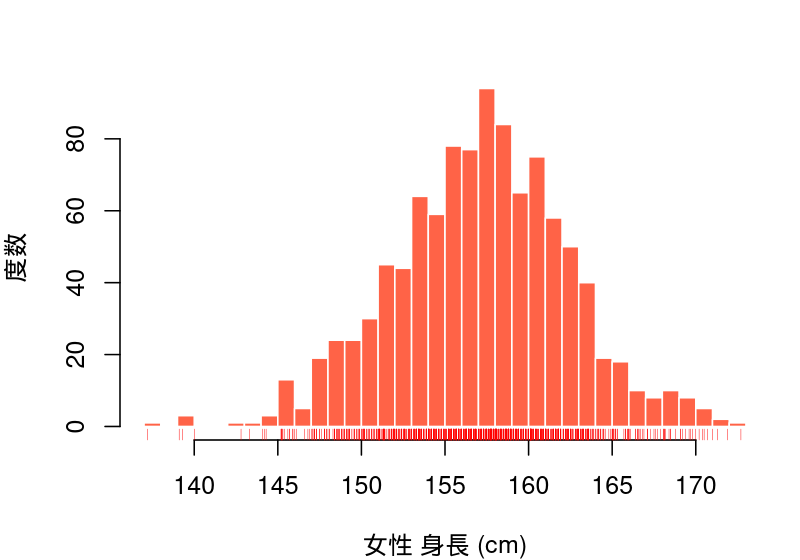
\includegraphics[width=\textwidth]{images/hist_f_ht.png}
        \caption{女性の身長}
        \label{fig:hist-f-ht}
    \end{subfigure}
    \hfill
    \begin{subfigure}[b]{0.48\textwidth}
        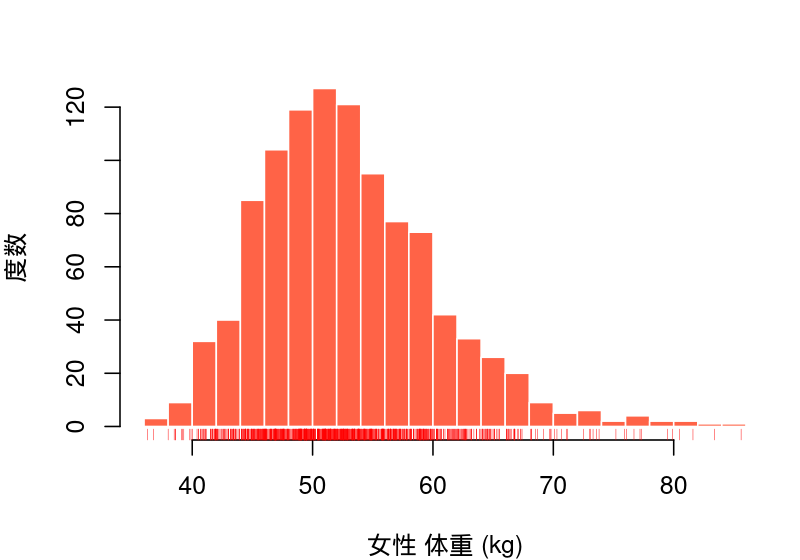
\includegraphics[width=\textwidth]{images/hist_f_wt.png}
        \caption{女性の体重}
        \label{fig:hist-f-wt}
    \end{subfigure}
    \caption{女性の身長・体重のヒストグラム}
    \label{fig:univariate-f-ht-wt}
\end{figure}
\vspace{-3.2em}

\begin{figure}[H]
    \centering
    \begin{subfigure}[b]{0.48\textwidth}
        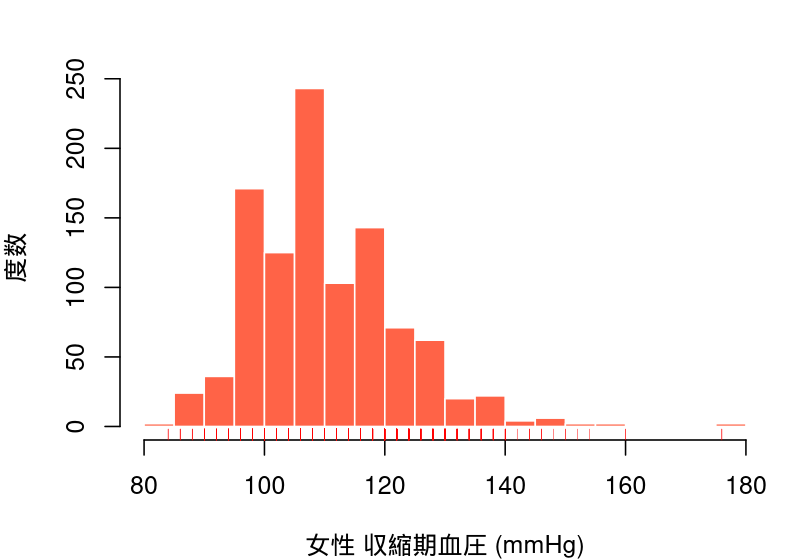
\includegraphics[width=\textwidth]{images/hist_f_sbp.png}
        \caption{女性の収縮期血圧}
        \label{fig:hist-f-sbp}
    \end{subfigure}
    \hfill
    \begin{subfigure}[b]{0.48\textwidth}
        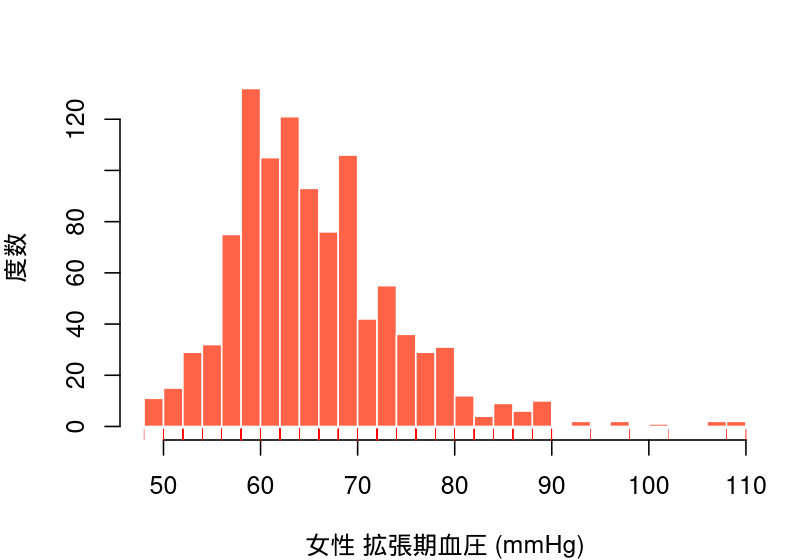
\includegraphics[width=\textwidth]{images/hist_f_dbp.png}
        \caption{女性の拡張期血圧}
        \label{fig:hist-f-dbp}
    \end{subfigure}
    \caption{女性の血圧のヒストグラム}
    \label{fig:univariate-f-bp}
\end{figure}
\vspace{-3.2em}
%% 要約統計量 ----------------------------------------------------
\begin{table}[htbp]
    \centering
    \caption{男女別の要約統計量}
    \label{tab:summary-mf}
    \begin{tabular}{lrrrrrrr}
        \toprule
        変数 & \multicolumn{1}{c}{$n$} & \multicolumn{1}{c}{平均} & \multicolumn{1}{c}{$SD$} & \multicolumn{1}{c}{中央値} & \multicolumn{1}{c}{Q1} & \multicolumn{1}{c}{Q3} & \multicolumn{1}{c}{IQR} \\
        \midrule
        \multicolumn{8}{c}{\textbf{男性（$n=602$）}} \\
        \midrule
        身長 (cm)   & 602 & 170.24 & 5.94  & 170.40 & 165.80 & 174.38 & 8.57 \\
        体重 (kg)   & 602 & 66.92  & 10.26 & 66.10  & 59.42  & 72.80  & 13.38 \\
        SBP (mmHg)  & 602 & 114.81 & 12.57 & 114.00 & 106.00 & 122.00 & 16.00 \\
        DBP (mmHg)  & 602 & 71.43  & 9.63  & 70.00  & 64.00  & 78.00  & 14.00 \\
        \midrule
        \multicolumn{8}{c}{\textbf{女性（$n=1038$）}} \\
        \midrule
        身長 (cm)   & 1038 & 157.16 & 5.22  & 157.40 & 153.90 & 160.60 & 6.70 \\
        体重 (kg)   & 1038 & 52.92  & 7.24  & 52.05  & 47.70  & 57.00  & 9.30 \\
        SBP (mmHg)  & 1038 & 110.86 & 12.11 & 110.00 & 102.00 & 118.00 & 16.00 \\
        DBP (mmHg)  & 1038 & 66.43  & 8.48  & 64.00  & 60.00  & 70.00  & 10.00 \\
        \bottomrule
    \end{tabular}
\end{table}

\subsubsection*{説明}
男女別の分析により、以下の特徴が確認された。

\begin{itemize}[nosep]
    \item \textbf{身長}: 男性の平均は170.24cm、女性の平均は157.16cmであり、約13cmの
          差がある。分布はいずれもほぼ正規分布に近い形状を示した。
    \item \textbf{体重}: 男性の平均は66.92kg、女性の平均は52.92kgであり、約14kgの
          差がある。男性の分布は女性に比べてやや右に裾が長い。
    \item \textbf{収縮期血圧（SBP）}: 男性の平均は114.81mmHg、女性の平均は110.86mmHg
          であり、男女差は約4mmHgと比較的小さい。IQRは男女とも16mmHgで同程度である。
    \item \textbf{拡張期血圧（DBP）}: 男性の平均は71.43mmHg、女性の平均は66.43mmHg
          であり、約5mmHgの差がみられた。女性のIQR（10mmHg）は男性（14mmHg）より
          小さく、分布がより集中している。
\end{itemize}

全体的に、男性のほうが身長・体重・血圧のいずれも高い値を示しており、標準偏差も
男性の方が大きい傾向にある。これは身体的特徴の性差を反映した結果と考えられる。

\clearpage

%% ============================================================
\section{問題2：データモデル}\label{sec:problem2}

%% ------------------------------------------------------------
\subsection{問題2(a)：投稿型SNSシステム}\label{sec:er-diagram}

投稿型SNSシステムを設計するために、以下の要件に基づいてER図を作成した。

\subsubsection{エンティティと属性の特定}
各エンティティとその属性を以下のように特定した。

\begin{itemize}[nosep]
    \item \textbf{ユーザー}: ユーザーID（PK）、名前、メールアドレス、作成日時
    \item \textbf{投稿}: 投稿ID（PK）、ユーザーID（FK）、投稿内容、投稿日時
    \item \textbf{いいね}: いいねID（PK）、ユーザーID（FK）、投稿ID（FK）、いいね日時
\end{itemize}

\subsubsection{エンティティ間の関係の定義}
エンティティ間のリレーションシップは以下の通りである。

\begin{itemize}[nosep]
    \item \textbf{ユーザー ─ 投稿}: 1人のユーザーは複数の投稿ができる（1対多）。
          投稿は必ず1人のユーザーに属する。
    \item \textbf{ユーザー ─ いいね}: 1人のユーザーは複数の投稿にいいねできる（1対多）。
          いいねは必ず1人のユーザーによるものである。
    \item \textbf{投稿 ─ いいね}: 1つの投稿は複数のいいねを受け取れる（1対多）。
          いいねは必ず1つの投稿に対するものである。
\end{itemize}

\subsubsection{ER図}
以上の分析に基づき、図\ref{fig:er-sns}にER図を示す。

\begin{figure}[htbp]
    \centering
    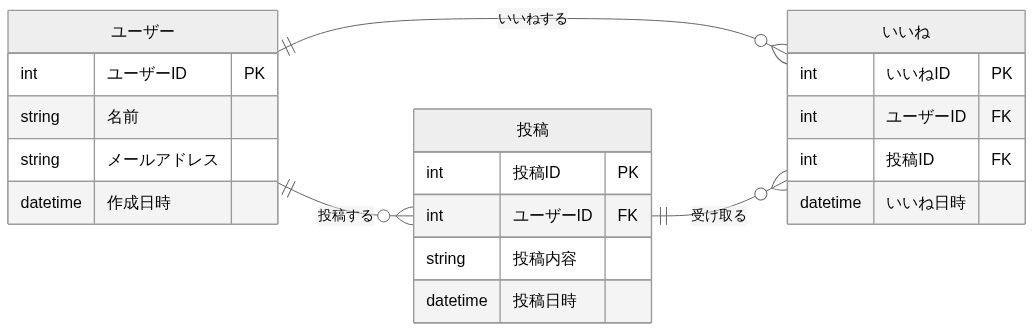
\includegraphics[width=\textwidth]{images/er_sns.png}
    \caption{投稿型SNSシステムのER図}
    \label{fig:er-sns}
\end{figure}

\subsubsection{説明}
本ER図では、3つのエンティティ（ユーザー、投稿、いいね）を定義した。
リレーションシップは全て1対多の関係であり、IE記法（crows-foot）で表現している。
「ユーザー」は「投稿」を通じてコンテンツを発信し、
「いいね」を通じて他者の投稿に反応する構造となっている。
これは典型的なSNSの最小構成を表現したものである。

%% ------------------------------------------------------------
\subsection{問題2(b)：dplyrを用いたデータの操作}\label{sec:db-script}

問題2(a)で設計したSNSデータベースのテーブルに対して、Rの\texttt{dplyr}パッケージを
用いた基本的なデータ操作の実装例を示す。最後の結合操作では\texttt{inner\_join}と
\texttt{left\_join}の両方を取り上げ、両者の違いを明示する。

\begin{itemize}[nosep]
    \item \textbf{tibbleの作成}: \texttt{ユーザー}テーブル、\texttt{投稿}テーブル、
          \texttt{いいね}テーブルを\texttt{tibble()}関数で作成した。各テーブルの
          カラム構成はER図の属性定義に従っている。
    \item \textbf{データの抽出}: \texttt{filter()}関数により、条件に合致する行のみを
          抽出できる。以下の例では、ユーザーIDが3のユーザーによる投稿のみを抽出している。
    \item \textbf{データの選択}: \texttt{select()}関数により、必要な列のみを選択できる。
          以下の例では、投稿IDと投稿内容の2列のみを取り出している。
    \item \textbf{データの追加}: \texttt{mutate()}関数により、既存の列から新しい列を
          作成できる。以下の例では、ユーザーの名前の文字数とメールアドレスのドメイン部分を
          新しい列として追加している。
    \item \textbf{データの集計}: \texttt{group\_by()}と\texttt{summarise()}を組み合わせる
          ことで、グループ別の集計が可能である。以下の例では、ユーザー別の投稿数と、
          各投稿に対するいいね数を集計している。
    \item \textbf{データの並べ替え}: \texttt{arrange()}関数により、指定した列の値に基づいて
          行を並べ替えられる。以下の例では、投稿日時の降順（新しい順）に並べ替えている。
    \item \textbf{データの結合}: \texttt{inner\_join()}と\texttt{left\_join()}により、
          複数のテーブルをキー列に基づいて結合できる。\texttt{inner\_join}は両方に
          キーが存在する行のみ、\texttt{left\_join}は左側テーブルの全行を保持する。
\end{itemize}

\subsubsection{実装}
%% R スクリプト -------------------------------------------------
\lstinputlisting[
    language=R,
    caption={問題2(b)のRスクリプト：dplyrによるデータ操作},
    label={lst:db-script}
]{code/task2-b.R}

\subsubsection{結果}
\lstinputlisting[
    language={},
    label={lst:db-script-result},
    numbers=none,
    basicstyle=\ttfamily\footnotesize
]{code/output_task2-b.txt}

\subsubsection{説明}
以上のスクリプトでは、問題2(a)で設計したSNSデータベースの3テーブル
（ユーザー、投稿、いいね）に対して、\texttt{dplyr}の主要な操作を
実装した。ユーザーテーブルには、\texttt{left\_join}と\texttt{inner\_join}
の違いを示すため、投稿を1件も行っていないユーザー（山田一郎）を
追加している。

\begin{itemize}[nosep]
    \item \textbf{tibbleの作成}: \texttt{tibble()}により、ER図で定義した各属性を
          カラムとするテーブルを作成した。日付型には\texttt{as.Date()}を用いて
          適切なデータ型を設定している。
    \item \textbf{filter（抽出）}: ユーザーIDが3の投稿のみを抽出する例を示した。
          これは実際のSNSで「特定ユーザーの投稿一覧」を表示する操作に相当する。
    \item \textbf{select（選択）}: 投稿IDと投稿内容のみを選択する例を示した。
          必要な列だけを抜き出す操作は、APIレスポンスの整形などで頻出する。
    \item \textbf{mutate（追加）}: \texttt{nchar()}で名前の文字数を、
          \texttt{sub()}でメールアドレスのドメイン部分を抽出し、新たな列として
          追加した。既存データから派生情報を生成する典型的なパターンである。
    \item \textbf{group\_by＋summarise（集計）}: ユーザー別の投稿数、および
          各投稿のいいね数を集計した。グループ化による集計は、SNSの分析基盤
          （ユーザーアクティビティの可視化など）で不可欠な操作である。
    \item \textbf{arrange（並べ替え）}: 投稿日時の降順で並べ替えることで、
          新しい投稿から順に表示するタイムライン機能を模した。
    \item \textbf{inner\_join / left\_join（結合）}: 投稿テーブルにユーザー名を
          \texttt{inner\_join}で結合し、さらに全ユーザーを残す\texttt{left\_join}
          の例も示した。\texttt{inner\_join}は両テーブルでキーが一致する行のみを
          返すのに対し、\texttt{left\_join}は左側のテーブルの全行を保持し、一致が
          ない列は\texttt{NA}となる。ユーザーID=6（山田一郎）は投稿が0件のため、
          \texttt{inner\_join}では除外され、\texttt{left\_join}では投稿情報が
          \texttt{NA}として表示される。これは、未投稿ユーザーの一覧を取得する
          といった実用的なシナリオで有用である。
\end{itemize}

これらの操作は、リレーショナルデータベースのSQLにおける
\texttt{SELECT}、\texttt{WHERE}、\texttt{GROUP BY}、\texttt{ORDER BY}、
\texttt{JOIN}などに相当し、\texttt{dplyr}を用いることでパイプライン
（\texttt{\%>\%}）による可読性の高いデータ処理が可能となることを確認した。

%% ------------------------------------------------------------
\subsection{問題2(c)：SNS投稿システムへの機能の追加}\label{sec:db-extension}

問題2(a)のSNSシステムに対して、ユーザーが投稿に対してコメントを書ける機能を追加する。
新たに\texttt{コメント}エンティティを導入し、ユーザーと投稿の両方に関連付ける。

\subsubsection{拡張ER図}
図\ref{fig:er-sns-extended}に、コメントエンティティを追加した全体のER図を示す。

\begin{figure}[htbp]
    \centering
    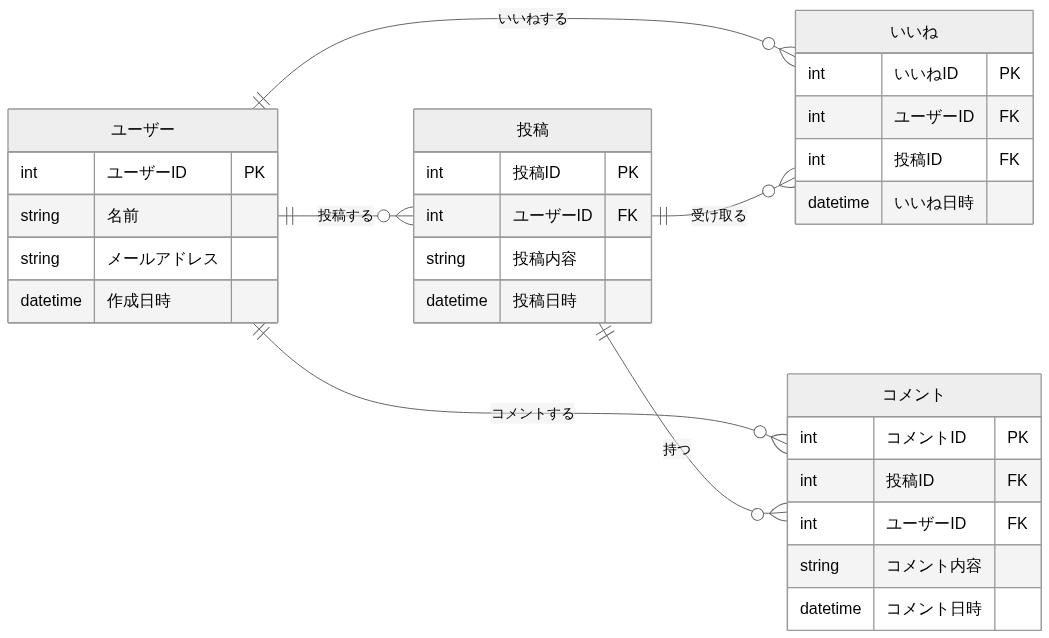
\includegraphics[width=\textwidth]{images/er_sns_extended.png}
    \caption{コメント機能を追加した拡張ER図}
    \label{fig:er-sns-extended}
\end{figure}

\subsubsection{追加テーブルの例}

\begin{table}[htbp]
    \centering
    \caption{コメントテーブルの例}
    \label{tab:comments}
    \begin{tabular}{rrrlr}
        \toprule
        コメントID & ユーザーID & 投稿ID & コメント内容 & コメント日時 \\
        \midrule
        1 & 2 & 1 & 私もR始めたばかりです！ & 2026-05-02 \\
        2 & 3 & 1 & 一緒に頑張りましょう & 2026-05-02 \\
        3 & 4 & 2 & dplyr便利ですよね & 2026-05-03 \\
        4 & 5 & 3 & ggplot2のグラフ見せてください & 2026-05-04 \\
        5 & 1 & 5 & 合格おめでとうございます！ & 2026-05-06 \\
        \bottomrule
    \end{tabular}
\end{table}

\subsubsection{説明}
\begin{itemize}[nosep]
    \item \textbf{追加内容}: ユーザーが投稿に対してテキストコメントを残せる
          \texttt{コメント}エンティティを追加した。属性はコメントID（PK）、
          投稿ID（FK）、ユーザーID（FK）、コメント内容、コメント日時である。
    \item \textbf{リレーションシップ}: 「ユーザー ─ コメント」は1対多（1人の
          ユーザーが複数コメント可能）、「投稿 ─ コメント」も1対多（1つの投稿が
          複数コメントを持てる）である。これにより、どのユーザーがどの投稿に
          どのようなコメントをいつ書いたかを全て追跡できる。
    \item \textbf{拡張の意図}: いいね機能だけでは表現できない「テキストによる
          フィードバック」を可能にすることで、SNSとしてのコミュニケーションの
          質を高めることが目的である。現実のSNS（Twitterのリプライ、Instagramの
          コメント等）でも同様の構造が採用されている。
\end{itemize}

\clearpage

%% ============================================================
\section{感想}\label{sec:impression}

今回の実験は二回目で\LaTeX を使ってレポートを作成した。最初はコマンドが多く、
コンパイルエラーにも戸惑ったが、徐々に慣れるにつれて文書構造と見た目を分離できる
\LaTeX の利点を実感した。特に、図表の参照番号や目次の自動生成、文献管理の
\texttt{thebibliography}環境などは、Wordでは難しい機能であり、長い文書を書く
際の強力なツールだと感じた。

また、問題2(a)と問題2(c)のER図作成には、Mermaid.jsを用いた。従来のドロー系
ツールでは図形を手作業で配置する必要があるが、Mermaid.jsはテキストベースの
DSLで記述できるため、ER図の構造そのものに集中できた。さらに、Pythonスクリプトで
mermaid.inkのAPIを呼び出し、PNG画像として自動出力するパイプラインを構築したことで、
図の修正や再生成が容易になった。コードで図を管理するという発想は非常に新鮮で、
今後のドキュメント作成にも積極的に活用したい。

全体を通して、Rによる統計処理・データ操作からデータモデリング、そして\LaTeX による
レポート執筆まで、一連のワークフローを経験できたことは大きな収穫であった。


\addcontentsline{toc}{section}{参考文献}
\begin{thebibliography}{9}

\bibitem{dplyr}
  H.~Wickham, R.~François, L.~Henry, K.~Müller, D.~Vaughan,
  \textit{dplyr: A Grammar of Data Manipulation},
  R package version 1.1.4,
  \url{https://dplyr.tidyverse.org/},
  \url{https://CRAN.R-project.org/package=dplyr},
  2024.

\bibitem{r4ds}
  H.~Wickham, G.~Grolemund,
  \textit{R for Data Science},
  2nd ed., O'Reilly Media,
  \url{https://r4ds.hadley.nz/},
  2023.

\bibitem{magrittr}
  S.~M.~Bache, H.~Wickham,
  \textit{magrittr: A Forward-Pipe Operator for R},
  R package version 2.0.3,
  \url{https://CRAN.R-project.org/package=magrittr},
  2022.

\bibitem{monad-moggi}
  E.~Moggi,
  ``Notions of computation and monads'',
  \textit{Information and Computation},
  vol.~93, no.~1, pp.~55--92, 1991.

\bibitem{er-ie}
  IDEF1X / IE Notation,
  ``Information Engineering Notation (Crow's Foot Integration Definition for Information Modeling)'',
  NIST, 1993.

\bibitem{r-base}
  R Core Team,
  \textit{R: A Language and Environment for Statistical Computing},
  R Foundation for Statistical Computing, Vienna, Austria,
  \url{https://www.R-project.org/},
  2024.

\end{thebibliography}
\end{document}
